\chapter{Resoluci\'{o} de Xarxes El\`{e}ctriques} \label{chap:nusos}

\index{metode@m\`{e}tode dels nusos}S'explica en aquest cap\'{\i}tol el
m\`{e}tode dels nusos, per a la resoluci\'{o} de xarxes el\`{e}ctriques.

\section{Introducci\'{o}}

Quan tenim una xarxa el\`{e}ctrica amb pocs components, sempre la podem resoldre f\`{a}cilment
utilitzant les lleis de Kirchhoff. No obstant, quan la xarxa t\'{e} molts components, quan est\`{a}
 molt mallada o quan hi ha acoblaments magn\`{e}tics entre diverses branques de la xarxa, \'{e}s millor
 emprar un m\`{e}tode sistem\`{a}tic per tal de resoldre-la, com ara el m\`{e}tode del nusos.

El m\`{e}tode dels nusos serveix per resoldre xarxes, tant de corrent
continu com de corrent altern, on les c\`{a}rregues estan definides pels
seus valors d'imped\`{a}ncia o d'admit\`{a}ncia; no \'{e}s \'{u}til per tant, per
resoldre problemes de flux de c\`{a}rregues, on el que es coneix \'{e}s la
potencia absorbida per les c\`{a}rregues.

Per utilitzar aquest m\`{e}tode, les branques de la xarxa han d'estar
formades per un dels seg\"{u}ents components: \vspace{-1.5mm}
\begin{dinglist}{'167}
   \item Font de tensi\'{o} en s\`{e}rie amb una imped\`{a}ncia.
   \item Font de corrent en para{\l.l}el amb una admit\`{a}ncia (l'admit\`{a}ncia pot ser nu{\l.l}a).
   \item Imped\`{a}ncia.
   \item Admit\`{a}ncia.
   \item Acoblament magn\`{e}tic entre branques.
   \item Transformador\footnote{Cal substituir el transformador pel seu circuit equivalent, format per imped\`{a}ncies i
   admit\`{a}ncies. Vegeu la Secci\'{o} \ref{sec:trafo_reg}.}
\end{dinglist}
\vspace{-1.5mm}

No \'{e}s possible tenir branques d'imped\`{a}ncia nu{\l.l}a (curt circuits) o
branques amb fonts de tensi\'{o} ideals (sense imped\`{a}ncia s\`{e}rie).
Aquesta limitaci\'{o} es pot superar, no obstant, substituint la
imped\`{a}ncia nu{\l.l}a per dues imped\`{a}ncies en s\`{e}rie i de valor
contrari, i introduint un nus fictici addicional en el punt d'uni\'{o}
d'aquestes dues noves imped\`{a}ncies. En la Figura
\vref{pic:branca_nula}
 es representa gr\`{a}ficament aquesta substituci\'{o}. \index{metode@m\`{e}tode dels nusos!branques d'imped\`{a}ncia
nu{\l.l}a}
\begin{figure}[htb]
\centering
   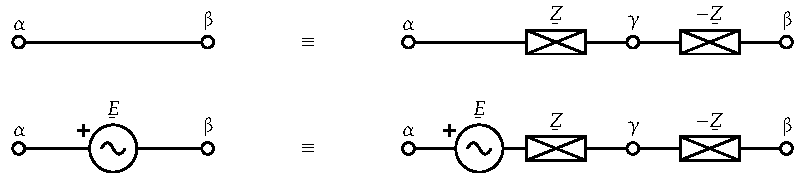
\includegraphics{Imatges/Cap-ResXarxElec-Branques-Z0.pdf}
\caption{Substituci\'{o} de branques d'imped\`{a}ncia nu{\l.l}a}
\label{pic:branca_nula}
\end{figure}

Per ajudar-nos en l'explicaci\'{o} d'aquest m\`{e}tode de resoluci\'{o} de xarxes, farem
\'{u}s de l'exemple de la Figura \vref{pic:metode_nusos}. Els valors dels components d'aquest
circuit s\'{o}n:
\begin{align*}
   \cmplx{E}_1 &= 200_{\angle 0\degree}\unit{V} & R_1 &= 10\unit{\ohm} &
   \cmplx{E}_2 &= 50_{\angle 0\degree}\unit{V}  & \cmplx{X}_2 &= \ju 20\unit{\ohm} &
   \cmplx{X}_3 &= \ju 5\unit{\ohm} \\
   R_4 &= 20\unit{\ohm} & \cmplx{J}_5 &= 4_{\angle 0\degree}\unit{A} &
   R_5 &= 10\unit{\ohm} & \cmplx{X}\ped{M} &= \ju 5\unit{\ohm}
\end{align*}

\begin{figure}[htb]
\vspace{-4mm} \centering
    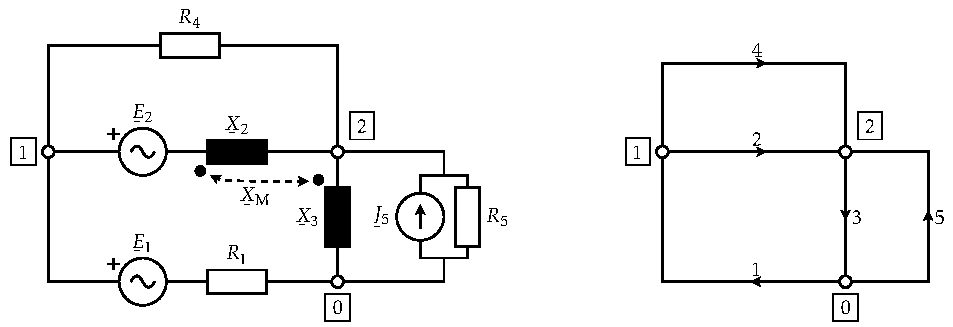
\includegraphics{Imatges/Cap-ResXarxElec-Circuit-Graf.pdf}
   \caption{Resoluci\'{o} de xarxes el\`{e}ctriques pel m\`{e}tode dels nusos} \label{pic:metode_nusos}
\end{figure}

\index{graf orientat}En primer lloc, a partir de la xarxa el\`{e}ctrica
cal representar el seu graf orientat, seguint els passos seg\"{u}ents
(Figura \vref{pic:metode_nusos}):
\begin{dingautolist}{'312}
   \item Es representen les connexions de les branques mitjan\c{c}ant l\'{\i}nies, sense dibuixar-hi cap component el\`{e}ctric.
   \item Es d\'{o}na un sentit a aquestes branques, dibuixant-hi fletxes. Aquestes fletxes representen els sentits assignats als corrents i a les difer\`{e}ncies de potencial entre nusos.
   \item Es numeren tots els nusos de forma consecutiva, comen\c{c}ant pel n\'{u}mero 0; el nus 0 s'anomena nus de potencial zero, o de refer\`{e}ncia.
\index{nus!de potencial zero}\index{nus!de refer\`{e}ncia}
   \item Es numeren totes les branques de forma consecutiva, comen\c{c}ant pel n\'{u}mero 1.
\end{dingautolist}

\index{metode@m\`{e}tode dels nusos!nombre de nusos}\index{metode@m\`{e}tode
dels nusos!nombre de branques}Es defineixen a continuaci\'{o} els dos
par\`{a}metres b\`{a}sics d'aquest m\`{e}tode, $n$ i $b$; aquests dos valors
defineixen les dimensions dels vectors i matrius que es veuran m\'{e}s
endavant:
\begin{list}{}
   {\setlength{\labelwidth}{7mm} \setlength{\leftmargin}{9mm} \setlength{\labelsep}{2mm}}
   \item[$n$:] Nombre de nusos de la xarxa, sense comptar el nus de refer\`{e}ncia.

   En el nostre exemple tenim:
   \[ n=2 \]

   \item[$b$:] Nombre de branques de la xarxa.

   En el nostre exemple tenim:
   \[ b=5 \]
\end{list}

\section{M\`{e}tode general de resoluci\'{o}}

\index{metode@m\`{e}tode dels nusos!cas general}Quan hi ha acoblaments
magn\`{e}tics entre branques de la xarxa hem d'utilitzar el m\`{e}tode
general de resoluci\'{o}, descrit a continuaci\'{o}.

En primer lloc, a partir dels valors dels components de la xarxa, formem les matrius i vectors seg\"{u}ents (es donen les seves dimensions entre claus):
\begin{list}{}
{\setlength{\labelwidth}{20mm} \setlength{\leftmargin}{22mm} \setlength{\labelsep}{2mm}}
   \item[$\boldsymbol{A}\{n\times b\}$:] \index{matriu!d'incid\`{e}ncia de nusos $\boldsymbol{A}$}Matriu d'incid\`{e}ncia de nusos. Cada columna representa una branca, en ordre creixent d'esquerra a dreta, i cada fila representa un nus (sense comptar el de refer\`{e}ncia) en ordre creixent, de dalt a baix. Cada branca del graf orientat omple la columna corresponent de la matriu $\boldsymbol{A}$ amb els valors 0, 1 \'{o} -1 segons el criteri seg\"{u}ent:
   \begin{list}{}
   {\setlength{\labelwidth}{7mm} \setlength{\leftmargin}{9mm} \setlength{\labelsep}{2mm}}
      \item[1:]  si la branca surt del nus.
      \item[-1:] si la branca va a para al nus.
      \item[0:]  si la branca ni surt ni va a parar al nus.
   \end{list}
   Els termes {"<}surt{">} i {"<}va a parar{">} s'han d'entendre segons les fletxes dibuixades en les branques del graf orientat. Les connexions al nus de refer\`{e}ncia, no apareixen en la matriu $\boldsymbol{A}$.

   En el nostre exemple tenim:
   \[
      \boldsymbol{A} = \left(\begin{array}{rrrrr} -1 & 1  & 0 &  1 & 0 \\  0 & -1 & 1 & -1 & -1
                   \end{array} \right)
   \]

   \item[$\mcmplx{Z}\ped{B}\{b\times b\}$:] \index{matriu!d'imped\`{a}ncies de branca $\mcmplx{Z}\ped{B}$}Matriu d'imped\`{a}ncies de branca. Els elements de la diagonal estan formats per les imped\`{a}ncies de les respectives branques, i els elements de fora de la diagonal estan formats per les imped\`{a}ncies dels acoblaments magn\`{e}tics entre cada parell de branques.

   Els acoblaments magn\`{e}tics poden ser positius o negatius, depenent
    de la posici\'{o} dels punts hom\`{o}legs de les induct\`{a}ncies i del sentit
    de les branques del graf orientat. L'acoblament \'{e}s positiu quan les
    fletxes de les dues branques acoblades es dirigeixen cap els seus punts
    hom\`{o}legs respectius, o quan les dues fletxes se n'allunyen; en canvi,
    l'acoblament \'{e}s negatiu quan una de les fletxes de les dues branques
    acoblades es dirigeix cap el seu punt hom\`{o}leg i l'altra se n'allunya.
    \index{acoblament magn\`{e}tic}

   En el nostre exemple tenim:
   \[
      \mcmplx{Z}\ped{B} = \begin{pmatrix}
            10 & 0 & 0 & 0 & 0 \\
            0 & \ju 20 & \ju 5 & 0 & 0 \\
            0 & \ju 5 & \ju 5 & 0 & 0 \\
            0 & 0 & 0 & 20 & 0 \\
            0 & 0 & 0 & 0 & 10
      \end{pmatrix}\unit{\ohm}
   \]

   \item[$\mcmplx{E}'\ped{B}\{b\}$:] \index{vector!de forces electromotrius $\mcmplx{E}'\ped{B}$}Vector columna de forces electromotrius de branca. Els elements d'aquest vector estan formats per les forces electromotrius de les fonts de tensi\'{o} de les respectives branques.

El signe de cada for\c{c}a electromotriu \'{e}s positiu, si el seu sentit coincideix amb el sentit de la fletxa de la branca corresponent del graf orientat, i negatiu en cas contrari.

   En el nostre exemple tenim:
   \[
      \mcmplx{E}'\ped{B} = \begin{pmatrix} 200 \\ -50 \\ 0 \\ 0 \\ 0 \end{pmatrix}\unit{V}
   \]

   \item[$\mcmplx{J}'\ped{B}\{b\}$:] \index{vector!d'intensivitats de branca $\mcmplx{J}'\ped{B}$}Vector columna d'intensivitats de branca. Els elements d'aquest vector estan formats per les intensivitats de les fonts de corrent de les respectives branques.

El signe de cada intensivitat \'{e}s positiu, si el seu sentit coincideix amb el sentit de la fletxa de la branca corresponent del graf orientat, i negatiu en cas contrari.

   En el nostre exemple tenim:
   \[
      \mcmplx{J}'\ped{B} = \begin{pmatrix} 0 \\ 0 \\ 0 \\ 0 \\ 4 \end{pmatrix}\unit{A}
   \]

\end{list}

A partir de les dades anteriors, formem ara les diverses matrius i
vectors que ens permetran resoldre la xarxa, aix\`{o} \'{e}s, trobar les
tensions de les branques i els corrents que hi circulen. Aquestes
matrius i vectors s\'{o}n (es donen les seves dimensions entre claus):

\begin{list}{}
{\setlength{\labelwidth}{20mm} \setlength{\leftmargin}{22mm} \setlength{\labelsep}{2mm}}
   \item[$\mcmplx{Y}\ped{B}\{b\times b\}$:] \index{matriu!d'admit\`{a}ncies de branca $\mcmplx{Y}\ped{B}$}Matriu d'admit\`{a}ncies de branca. Est\`{a} definida per la relaci\'{o} seg\"{u}ent:
   \begin{equation}
      \mcmplx{Y}\ped{B} = \mcmplx{Z}\ped{B}^{-1}
   \end{equation}

   En el nostre exemple tenim:
   \[
      \mcmplx{Y}\ped{B} = \begin{pmatrix}
            10 & 0 & 0 & 0 & 0 \\
            0 & \ju 20 & \ju 5 & 0 & 0 \\
            0 & \ju 5 & \ju 5 & 0 & 0 \\
            0 & 0 & 0 & 20 & 0 \\
            0 & 0 & 0 & 0 & 10
      \end{pmatrix} ^{-1} =
      \begin{pmatrix}
            \frac{1}{10} & 0 & 0 & 0 & 0 \\
            0 & -\ju\frac{1}{15} & \ju\frac{1}{15} & 0 & 0 \\
            0 & \ju\frac{1}{15} & -\ju\frac{4}{15} & 0 & 0 \\
            0 & 0 & 0 & \frac{1}{20} & 0 \\
            0 & 0 & 0 & 0 & \frac{1}{10}
      \end{pmatrix}\unit{S}
   \]

   \item[$\mcmplx{J}\ped{B}\{b\}$:] \index{vector!d'intensivitats equivalents de branca $\mcmplx{J}\ped{B}$}Vector columna d'intensivitats equivalents de branca. Est\`{a} definit per la relaci\'{o} seg\"{u}ent:
   \begin{equation}
      \mcmplx{J}\ped{B} = \mcmplx{J}'\ped{B}  + \mcmplx{Y}\ped{B} \,\mcmplx{E}'\ped{B}
   \end{equation}

   En el nostre exemple tenim:
   \[
      \mcmplx{J}\ped{B} =
      \begin{pmatrix} 0 \\ 0 \\ 0 \\ 0 \\ 4 \end{pmatrix} +
      \begin{pmatrix}
            \frac{1}{10} & 0 & 0 & 0 & 0 \\
            0 & -\ju\frac{1}{15} & \ju\frac{1}{15} & 0 & 0 \\
            0 & \ju\frac{1}{15} & -\ju\frac{4}{15} & 0 & 0 \\
            0 & 0 & 0 & \frac{1}{20} & 0 \\
            0 & 0 & 0 & 0 & \frac{1}{10}
      \end{pmatrix} \cdot
      \begin{pmatrix} 200 \\ -50 \\ 0 \\ 0 \\ 0 \end{pmatrix} =
      \begin{pmatrix} 20 \\ \ju\frac{10}{3} \\ -\ju\frac{10}{3} \\ 0 \\ 4 \end{pmatrix}
     \unit{A}
   \]

   \item[$\mcmplx{Y}\ped{N}\{n\times n\}$:] \index{matriu!d'admit\`{a}ncies de nus $\mcmplx{Y}\ped{N}$}Matriu d'admit\`{a}ncies de nus. Est\`{a} definida per la relaci\'{o} seg\"{u}ent:
   \begin{equation}
      \mcmplx{Y}\ped{N} = \boldsymbol{A} \mcmplx{Y}\ped{B}
      \transp{\boldsymbol{A}}
   \end{equation}

   En el nostre exemple tenim:
   \[ \begin{split}
      \mcmplx{Y}\ped{N} &=
      \left(\begin{array}{rrrrr} -1 & 1  & 0 &  1 & 0 \\  0 & -1 & 1 & -1 & -1
      \end{array}\right) \cdot
      \begin{pmatrix}
            \frac{1}{10} & 0 & 0 & 0 & 0 \\
            0 & -\ju\frac{1}{15} & \ju\frac{1}{15} & 0 & 0 \\
            0 & \ju\frac{1}{15} & -\ju\frac{4}{15} & 0 & 0 \\
            0 & 0 & 0 & \frac{1}{20} & 0 \\
            0 & 0 & 0 & 0 & \frac{1}{10}
      \end{pmatrix} \cdot
      \left(\begin{array}{rr} -1 & 0 \\ 1  & -1 \\  0 & 1 \\ 1 & -1 \\ 0 & -1
      \end{array}\right) = \\
       &=
      \frac{1}{60} \cdot \begin{pmatrix}
            9 - \ju 4 & -3 + \ju 8 \\
            3 + \ju 8 & 9 - \ju 28
      \end{pmatrix}\unit{S}
   \end{split}  \label{eq:yn}
   \]

   \item[$\mcmplx{J}\ped{N}\{n\}$:] \index{vector!d'intensivitats de nus $\mcmplx{J}\ped{N}$}Vector columna d'intensivitats de nus. Est\`{a} definit per la relaci\'{o} seg\"{u}ent:
   \begin{equation}
      \mcmplx{J}\ped{N} = - \boldsymbol{A} \,\mcmplx{J}\ped{B}
   \end{equation}

   En el nostre exemple tenim:
   \[
      \mcmplx{J}\ped{N} = -
      \left(\begin{array}{rrrrr} -1 & 1  & 0 &  1 & 0 \\  0 & -1 & 1 & -1 & -1
      \end{array}\right) \cdot
      \begin{pmatrix} 20 \\ \ju\frac{10}{3} \\ -\ju\frac{10}{3} \\ 0 \\ 4 \end{pmatrix}
      =
      \frac{1}{3} \cdot \begin{pmatrix}
            60 - \ju 10 \\
            12 + \ju 20
      \end{pmatrix}\unit{A}
   \]

   \item[$\mcmplx{V}\ped{N}\{n\}$:] \index{vector!de potencials de nus $\mcmplx{V}\ped{N}$}Vector columna de potencials de nus. Est\`{a} definit per la relaci\'{o} seg\"{u}ent:
   \begin{equation}
      \mcmplx{Y}\ped{N} \mcmplx{V}\ped{N} = \mcmplx{J}\ped{N} \quad\rightarrow\quad
      \mcmplx{V}\ped{N} = \mcmplx{Y}\ped{N}^{-1} \mcmplx{J}\ped{N} \label{eq:vn}
   \end{equation}

   Els elements d'aquest vector s\'{o}n els potencials de cada nus de la xarxa respecte del nus de refer\`{e}ncia.

   En el nostre exemple tenim:
   \[
      \mcmplx{V}\ped{N} = 60 \cdot
      \begin{pmatrix}
            9 - \ju 4 & -3 + \ju 8 \\
            3 + \ju 8 & 9 - \ju 28
      \end{pmatrix} ^{-1} \cdot
      \frac{1}{3} \cdot \begin{pmatrix}
            60 - \ju 10 \\
            12 + \ju 20
      \end{pmatrix}
      =
      \frac{1}{101} \cdot \begin{pmatrix}
            15430 + \ju 2295 \\
            3390 + \ju 2085
      \end{pmatrix}\unit{V}
      \label{eq:vn_exemp}
   \]

   \item[$\mcmplx{U}\ped{B}\{b\}$:] \index{vector!de tensions de branca $\mcmplx{U}\ped{B}$}Vector columna de tensions de branca. Est\`{a} definit per la relaci\'{o} seg\"{u}ent:
   \begin{equation}
      \mcmplx{U}\ped{B} = \transp{\boldsymbol{A}} \mcmplx{V}\ped{N} \label{eq:ur}
   \end{equation}

   Aquesta \'{e}s la soluci\'{o} buscada pel que fa a les tensions de les branques de la xarxa.

   En el nostre exemple tenim:
   \[
      \mcmplx{U}\ped{B} =
      \left(\begin{array}{rr} -1 & 0 \\ 1  & -1 \\  0 & 1 \\ 1 & -1 \\ 0 & -1
      \end{array}\right) \cdot
      \frac{1}{101} \cdot \begin{pmatrix}
            15430 + \ju 2295 \\
            3390 + \ju 2085
      \end{pmatrix} =
      \frac{1}{101} \cdot \begin{pmatrix}
            -15430 - \ju 2295 \\
            12040 + \ju 210  \\
            3390 + \ju 2085 \\
            12040 + \ju 210  \\
            -3390 - \ju 2085
      \end{pmatrix}\unit{V}
   \]

   \item[$\mcmplx{I}\ped{B}\{b\}$:] \index{vector!de corrents de branca $\mcmplx{I}\ped{B}$} Vector columna de corrents de branca. Est\`{a} definit per la relaci\'{o} seg\"{u}ent:
   \begin{equation}
      \mcmplx{I}\ped{B} = \mcmplx{Y}\ped{B} \,\mcmplx{U}\ped{B} + \mcmplx{J}\ped{B} \label{eq:ir}
   \end{equation}

   Aquesta \'{e}s la soluci\'{o} buscada pel que fa als corrents de les branques de la xarxa.

   En el nostre exemple tenim:
\end{list}
\[
   \mcmplx{I}\ped{B} =
   \begin{pmatrix}
         \frac{1}{10} & 0 & 0 & 0 & 0 \\
         0 & -\ju\frac{1}{15} & \ju\frac{1}{15} & 0 & 0 \\
         0 & \ju\frac{1}{15} & -\ju\frac{4}{15} & 0 & 0 \\
         0 & 0 & 0 & \frac{1}{20} & 0 \\
         0 & 0 & 0 & 0 & \frac{1}{10}
   \end{pmatrix} \cdot
   \frac{1}{101} \cdot \begin{pmatrix}
         -15430 - \ju 2295 \\
         12040 + \ju 210  \\
         3390 + \ju 2085 \\
         12040 + \ju 210  \\
         -3390 - \ju 2085
   \end{pmatrix}
   + \begin{pmatrix} 20 \\ \ju\frac{10}{3} \\ -\ju\frac{10}{3} \\ 0 \\ 4 \end{pmatrix} =
   \frac{1}{202} \cdot \begin{pmatrix}
         954 - \ju 459 \\
      -250 - \ju 480  \\
      1084 - \ju 876 \\
         1204 + \ju 21  \\
         130 - \ju 417
   \end{pmatrix}\unit{A}
\]

Es resumeixen finalment, els passos a seguir per tal de resoldre una
xarxa el\`{e}ctrica, mitjan\c{c}ant el m\`{e}tode dels nusos:
\begin{dingautolist}{'312}
   \item Es representa el graf orientat associat a la xarxa, i es numeren tots els seus nusos i totes les seves branques.
   \item A partir del graf orientat i dels elements de la xarxa, es formen les matrius $\boldsymbol{A}$ i $\mcmplx{Z}\ped{B}$, i els vectors $\mcmplx{E}\ped{B}'$ i $\mcmplx{J}\ped{B}'$.
   \item Es calculen les matrius $\mcmplx{Y}\ped{B}$ i $\mcmplx{Y}\ped{N}$, i els vectors $\mcmplx{J}\ped{B}$ i $\mcmplx{J}\ped{N}$.
   \item Finalment, es calculen els vectors $\mcmplx{V}\ped{N}$, $\mcmplx{U}\ped{B}$ i $\mcmplx{I}\ped{B}$.
\end{dingautolist}

\begin{exemple}
Es tracte de resoldre la xarxa seg\"{u}ent pel m\`{e}tode dels nusos; cal
tenir en compte que a m\'{e}s de la c\`{a}rrega Q8, els generadors G1, G2 i
G3 tamb\'{e} estan units a terra (nus 0 de refer\`{e}ncia), i que hi ha un
acoblament magn\`{e}tic M entre les l\'{\i}nies L5 i L6. Es calcular\`{a} tamb\'{e}
la pot\`{e}ncia cedida pels tres generadors G1, G2 i G3, la pot\`{e}ncia
absorbida per la c\`{a}rrega Q8 i la pot\`{e}ncia perduda en la resta de
components de la xarxa.
\begin{figure}[htb]
\vspace{3mm} \centering
   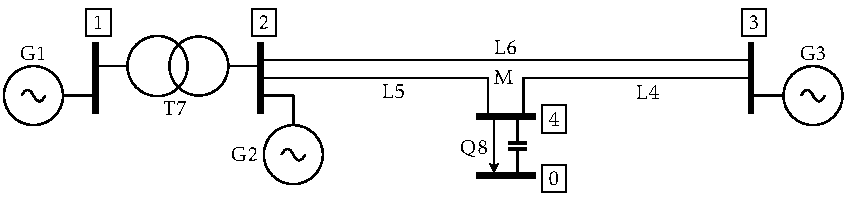
\includegraphics{Imatges/Cap-ResXarxElec-Exemple-Circuit.pdf}
\end{figure}

Els valors dels components d'aquesta xarxa, expressats en p.u.\ s\'{o}n:
\begin{align*}
   G1 &:\; \cmplx{e}_1 = 1{,}1 \qquad\qquad\;\;\, \cmplx{z}_1 = \ju 0{,}25 & L4 &:\; \cmplx{z}_4 = \ju 0{,}10 & T7 &:\; \cmplx{z}_7 = \ju 0{,}16 \quad\quad m_7=1:1\\
   G2 &:\; \cmplx{e}_2 = 1{,}05+\ju0{,}10 \quad \cmplx{z}_2 = \ju 0{,}20 & L5 &:\; \cmplx{z}_5 = \ju 0{,}405  & Q8 &:\; \cmplx{j}_8 = 2-\ju0{,}9 \quad \cmplx{z}_8 = -\ju25 \\
   G3 &:\; \cmplx{e}_3 = 1{,}08+\ju0{,}12 \quad \cmplx{z}_3 = \ju 0{,}25 & L6 &:\; \cmplx{z}_6 = \ju 0{,}50 & M &:\; \cmplx{x}_M = \ju0{,}05\; \text{(entre L5 i L6)}
\end{align*}

Comen\c{c}arem dibuixant el graf orientat associat a la xarxa, i formant la matriu $\boldsymbol{A}$.
\begin{figure}[htb]
\hfill
\begin{minipage}[c]{7cm}
    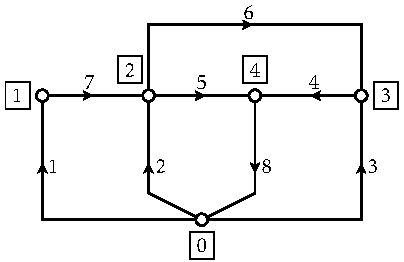
\includegraphics{Imatges/Cap-ResXarxElec-Exemple-Graf.pdf}
\end{minipage}
\hfill
\begin{minipage}[c]{9cm}
   \[
   \boldsymbol{A} = \left( \begin{array}{rrrrrrrr}
     -1 & 0 & 0 & 0 & 0 & 0 & 1 & 0 \\
     0 & -1 & 0 & 0 & 1 & 1 & -1 & 0 \\
     0 & 0 & -1 & 1 & 0 & -1 & 0 & 0 \\
     0 & 0 & 0 & -1 & -1 & 0 & 0 & 1
   \end{array}\right)
   \]
\end{minipage}
\hfill{}
\end{figure}

Formem a continuaci\'{o} la matriu $\mcmplx{Z}\ped{B}$ i els vectors $\mcmplx{J}\ped{B}'$ i $\mcmplx{E}\ped{B}'$ (tots els valors en p.u.):
\[
   \mcmplx{Z}\ped{B} = \ju \cdot
   \begin{pmatrix}
     0{,}25 & 0 & 0 & 0 & 0 & 0 & 0 & 0 \\
     0 & 0{,}20 & 0 & 0 & 0 & 0 & 0 & 0 \\
     0 & 0 & 0{,}25 & 0 & 0 & 0 & 0 & 0 \\
     0 & 0 & 0 & 0{,}10 & 0 & 0 & 0 & 0 \\
     0 & 0 & 0 & 0 & 0{,}405 & 0{,}05 & 0 & 0 \\
     0 & 0 & 0 & 0 & 0{,}05 & 0{,}50 & 0 & 0 \\
     0 & 0 & 0 & 0 & 0 & 0 & 0{,}16 & 0 \\
     0 & 0 & 0 & 0 & 0 & 0 & 0 & -25
   \end{pmatrix}
   \;\;
   \mcmplx{J}\ped{B}' =
   \begin{pmatrix}
    0 \\
    0 \\
    0 \\
    0 \\
    0 \\
    0 \\
    0 \\
    2 - \ju 0{,}9
   \end{pmatrix}
   \;\;
   \mcmplx{E}\ped{B}' =
   \begin{pmatrix}
    1{,}1 \\
    1{,}05 + \ju 0{,}10 \\
    1{,}08 + \ju 0{,}12 \\
    0 \\
    0 \\
    0 \\
    0 \\
    0
   \end{pmatrix}
\]

Calculem ara la matriu $\mcmplx{Y}\ped{B}=\mcmplx{Z}\ped{B}^{-1}$ i el vector $\mcmplx{J}\ped{B} = \mcmplx{J}\ped{B}' + \mcmplx{Y}\ped{B} \,\mcmplx{E}\ped{B}'$  (tots els valors en p.u.):
\[
   \mcmplx{Y}\ped{B} = \ju \cdot
   \begin{pmatrix}
     -4 & 0 & 0 & 0 & 0 & 0 & 0 & 0 \\
     0 & -5 & 0 & 0 & 0 & 0 & 0 & 0 \\
     0 & 0 & -4 & 0 & 0 & 0 & 0 & 0 \\
     0 & 0 & 0 & -10 & 0 & 0 & 0 & 0 \\
     0 & 0 & 0 & 0 & -2{,}5 & 0{,}25 & 0 & 0 \\
     0 & 0 & 0 & 0 & 0{,}25 & -2{,}025 & 0 & 0 \\
     0 & 0 & 0 & 0 & 0 & 0 & -6{,}25 & 0 \\
     0 & 0 & 0 & 0 & 0 & 0 & 0 & 0{,}04
   \end{pmatrix}
   \qquad
   \mcmplx{J}\ped{B} =
   \begin{pmatrix}
    -\ju 4{,}4 \\
    0{,}5 - \ju 5{,}25 \\
    0{,}48 - \ju 4{,}32 \\
    0 \\
    0 \\
    0 \\
    0 \\
    2 - \ju 0{,}9
   \end{pmatrix}
\]

Continuem amb el c\`{a}lcul de la matriu $\mcmplx{Y}\ped{N} =
\boldsymbol{A} \mcmplx{Y}\ped{B} \transp{\boldsymbol{A}}$ i dels
vectors $\mcmplx{J}\ped{N} = - \boldsymbol{A} \mcmplx{J}\ped{B}$ i
$\mcmplx{V}\ped{N} = \mcmplx{Y}\ped{N}^{-1} \mcmplx{J}\ped{N}$ (tots
els valors en p.u.):
\[
   \mcmplx{Y}\ped{N} = \ju \cdot
   \begin{pmatrix}
     -10{,}25 & 6{,}25 & 0 & 0 \\
     6{,}25 & -15{,}275 & 1{,}775 & 2{,}25 \\
     0 & 1{,}775 & -16{,}025 & 10{,}25 \\
     0 & 2{,}25 & 10{,}25 & -12{,}46
   \end{pmatrix}
   \;\;
   \mcmplx{J}\ped{N} =
   \begin{pmatrix}
    -\ju 4{,}4 \\
    0{,}5 - \ju 5{,}25 \\
    0{,}48 - \ju 4{,}32 \\
    -2 + \ju 0{,}9
   \end{pmatrix}
   \;\;
   \mcmplx{V}\ped{N} =
   \left(\begin{array}{l}
    1{,}0494_{\angle -1{,}4909\degree} \\
    1{,}0175_{\angle -2{,}5224\degree} \\
    0{,}9727_{\angle -10{,}3558\degree} \\
    0{,}9512_{\angle -19{,}1752\degree}
   \end{array}\right)
\]

Finalment, calculem les tensions i els corrents de les branques,
mitjan\c{c}ant els vectors $\mcmplx{U}\ped{B} = \transp{\boldsymbol{A}}
\mcmplx{V}\ped{N}$ i $\mcmplx{I}\ped{B} =  \mcmplx{Y}\ped{B}\,
\mcmplx{U}\ped{B} + \mcmplx{J}\ped{B}$ (tots els valors en p.u.):
\[
   \mcmplx{U}\ped{B} =
   \left(\begin{array}{l}
     1{,}0494_{\angle 178{,}5091\degree} \\
     1{,}0175_{\angle 177{,}4776\degree} \\
     0{,}9727_{\angle 169{,}6442\degree} \\
     0{,}1495_{\angle 67{,}0039\degree} \\
     0{,}2925_{\angle 66{,}2049\degree} \\
     0{,}1431_{\angle 65{,}3702\degree} \\
     0{,}0370_{\angle 28{,}1937\degree} \\
     0{,}9512_{\angle -19{,}1752\degree}
   \end{array}\right)
   \qquad
   \mcmplx{I}\ped{B} =
   \left(\begin{array}{l}
     0{,}2312_{\angle -61{,}8063\degree} \\
     0{,}7431_{\angle -13{,}0406\degree} \\
     1{,}2782_{\angle -22{,}6715\degree} \\
     1{,}4946_{\angle -22{,}9961\degree} \\
     0{,}6955_{\angle -23{,}7522\degree} \\
     0{,}2166_{\angle -24{,}9115\degree} \\
     0{,}2312_{\angle -61{,}8063\degree} \\
     2{,}1901_{\angle -23{,}2362\degree}
   \end{array}\right)
\]

Calcularem ara la pot\`{e}ncia cedida pels tres generadors G1, G2 i G3, i la pot\`{e}ncia absorbida per la c\`{a}rrega Q8. Cal tenir en compte que per calcular les pot\`{e}ncies cedides per generadors, els vectors que representen la for\c{c}a electromotriu del generador i el corrent que travessa el generador han de tenir el mateix sentit de refer\`{e}ncia; aix\'{\i} mateix, per calcular les pot\`{e}ncies absorbides per c\`{a}rregues, els vectors que representen la caiguda de tensi\'{o} a la c\`{a}rrega i el corrent que travessa la c\`{a}rrega han de tenir el mateix sentit de refer\`{e}ncia. Amb aquestes consideracions, tenim:
\begin{alignat*}{3}
   \cmplx{s}\ped{G1} &= \cmplx{e}\ped{1} \, \mcmplx{I}\ped{B}^*(1) &&= 1{,}1 \cdot
    0{,}2312_{\angle 61{,}8063\degree} &&= 0{,}1201 + \ju 0{,}2241 \unit{p.u.} \\
   \cmplx{s}\ped{G2} &= \cmplx{e}\ped{2} \, \mcmplx{I}\ped{B}^*(2) &&=
   (1{,}05 + \ju 0{,}10) \cdot 0{,}7431_{\angle 13{,}0406\degree} &&=
   0{,}7433 + \ju 0{,}2484\unit{p.u.}   \\
   \cmplx{s}\ped{G3} &= \cmplx{e}\ped{3} \, \mcmplx{I}\ped{B}^*(3) &&=
   (1{,}08 + \ju 0{,}12) \cdot 1{,}2782_{\angle 22{,}6715\degree} &&=
   1{,}2146 + \ju 0{,}6736\unit{p.u.}   \\
   \cmplx{s}\ped{Q8} &= \mcmplx{U}\ped{B}(8) \, \mcmplx{I}\ped{B}^*(8) &&=
   0{,}9512_{\angle -19{,}1752\degree} \cdot 2{,}1901_{\angle          23{,}2362\degree}     &&= 2{,}0780 + \ju 0{,}1475\unit{p.u.}
\end{alignat*}

La difer\`{e}ncia entre les pot\`{e}ncies generades i la pot\`{e}ncia absorbida, \'{e}s la pot\`{e}ncia perduda en la resta de components de la xarxa:
\[
   \cmplx{s}\ped{G1} + \cmplx{s}\ped{G2} + \cmplx{s}\ped{G3} -
   \cmplx{s}\ped{Q8} = \ju 0{,}9986\unit{p.u.}
\]
\end{exemple}


\section{M\`{e}tode particular de resoluci\'{o} sense acoblaments magn\`{e}tics}
\index{metode@m\`{e}tode dels nusos!cas particular!sense acoblaments
magn\`{e}tics}

Quan no hi ha acoblaments magn\`{e}tics entre branques de la xarxa, la matriu $\mcmplx{Y}\ped{N}\{n \times n\}$ i el vector $\mcmplx{J}\ped{N}\{n\}$ es poden formar de manera directa, a partir dels components de la xarxa i del seu graf orientat associat.

Per ajudar-nos en l'explicaci\'{o} d'aquest m\`{e}tode simplificat, farem \'{u}s
del mateix exemple de la Figura \vref{pic:metode_nusos}, per\`{o}
suposant que no hi ha acoblament magn\`{e}tic entre les branques 2 i 3
($\cmplx{X}\ped{M}=0$).

La matriu $\mcmplx{Y}\ped{N}\{n \times n\}$ i el vector $\mcmplx{J}\ped{N}\{n\}$ es formen tal com es descriu a continuaci\'{o}:

\begin{list}{}
   {\setlength{\labelwidth}{20mm} \setlength{\leftmargin}{22mm} \setlength{\labelsep}{2mm}}

   \item[$\mcmplx{Y}\ped{N}\{n \times n\}$:] \index{matriu!d'admit\`{a}ncies de nus $\mcmplx{Y}\ped{N}$}Matriu d'admit\`{a}ncies de nus. Els elements de la diagonal estan formats per la suma de les admit\`{a}ncies de les branques que incideixen en cada nus.
   Els elements de fora de la diagonal estan formats per la suma, canviada de signe, de les admit\`{a}ncies de les branques que estan connectades entre cada parella de nusos.

   En el nostre exemple tenim:
   \[
      \mcmplx{Y}\ped{N} =
      \begin{pmatrix}
            \frac{1}{20} + \frac{1}{\ju 20} +  \frac{1}{10} &
            -\left[\frac{1}{20} + \frac{1}{\ju 20}\right] \\
            -\left[\frac{1}{20} + \frac{1}{\ju 20}\right]  &
            \frac{1}{20} + \frac{1}{\ju 20} +  \frac{1}{\ju 5} + \frac{1}{10}
      \end{pmatrix} =
      \frac{1}{20} \cdot \begin{pmatrix}
            3 - \ju  & -1 + \ju \\ -1 + \ju & 3 - \ju 5
      \end{pmatrix}\unit{S}
   \]

   \item[$\mcmplx{J}\ped{N}\{n\}$:] \index{vector!d'intensivitats de nus $\mcmplx{J}\ped{N}$}Vector
d'intensivitats de nus. Cada element d'aquest vector est\`{a} format per la suma de
les intensivitats, degudes a les fonts de corrent i a les fonts de tensi\'{o}, de les
branques que incideixen en cada nus; el signe de cada intensivitat \'{e}s positiu si el
corrent va cap al nus, i negatiu si se n'allunya. Les fonts de tensi\'{o} han de
transformar-se en fonts de corrent, utilitzant l'equaci\'{o} \eqref{eq:Thevenin-Norton} de
la p\`{a}gina \pageref{eq:Thevenin-Norton}.

   En el nostre exemple tenim:
   \[
      \mcmplx{J}\ped{N} =
      \begin{pmatrix}
            \frac{50}{\ju 20} +  \frac{200}{10} \\
            - \frac{50}{\ju 20} + 4
      \end{pmatrix} =
      \frac{1}{2} \cdot \begin{pmatrix}
            40 - \ju 5 \\
            8 + \ju 5
      \end{pmatrix}\unit{A}
   \]

\end{list}

\index{vector!de potencials de nus $\mcmplx{V}\ped{N}$}Finalment,
trobem el vector de potencials de nus $\mcmplx{V}\ped{N}\{n\}$, tal
com  hem fet en l'apartat anterior, aplicant l'equaci\'{o} \eqref{eq:vn}

En el nostre exemple tenim:
\[
   \mcmplx{V}\ped{N} =
   20 \cdot \begin{pmatrix}
         3 - \ju  & -1 + \ju \\ -1 + \ju & 3 - \ju 5
   \end{pmatrix} ^{-1} \cdot
   \frac{1}{2} \cdot \begin{pmatrix}
         40 - \ju 5 \\
         8 + \ju 5
   \end{pmatrix} =
   \frac{1}{17} \cdot \begin{pmatrix}
         2450 + \ju 535 \\ 540  + \ju 545
   \end{pmatrix}\unit{V}
\]

Si volem trobar ara de forma sistem\`{a}tica, totes les tensions i tots
els corrents i  de les branques de la xarxa, haurem d'utilitzar
l'equaci\'{o} \eqref{eq:ur} de la p\`{a}gina \pageref{eq:ur} i l'equaci\'{o}
\eqref{eq:ir} de la p\`{a}gina \pageref{eq:ir}; aix\`{o} vol dir que haurem
de formar les matrius $\boldsymbol{A}$ i $\mcmplx{Y}\ped{B}$ i el
vector $\mcmplx{J}\ped{B}$. No obstant, si \'{u}nicament estem
interessats en algun corrent o en alguna tensi\'{o} de branca, podem
resoldre el problema aplicant les lleis de Kirchhoff a les branques
que ens interessin.


\begin{exemple}
A partir del circuit de la Figura \vref{pic:metode_nusos}, amb
$\cmplx{X}\ped{M}=0$, es tracta de trobar els corrents que circulen
per les branques 2 i 5.

Partint dels potencials dels nusos 1 i 2 calculats anteriorment, i
aplicant les lleis de Kirchhoff a les branques 2 i 5 tenim:
\begin{align*}
   \cmplx{I}_2 &= \frac{-\cmplx{E}_2 + [\mcmplx{V}\ped{N}(1) - \mcmplx{V}\ped{N}(2)]}
                  {\cmplx{X}_2} = \frac{-50 + \frac{2450+\ju 535 -540
                  - \ju 545}{17}} {\ju 20} = \frac{-1 - \ju 106}{34}\unit{A} \\[1.5ex]
   \cmplx{I}_5 &=  \frac{- \mcmplx{V}\ped{N}(2)}{R_5}  + \cmplx{J}_5 =
                  \frac{\frac{-540 - \ju 545}{17}}{10} + 4 =
                  \frac{28 - \ju 109}{34}\unit{A}
\end{align*}

\end{exemple}

\section{M\`{e}tode particular de resoluci\'{o} amb acoblaments magn\`{e}tics}
\index{metode@m\`{e}tode dels nusos!cas particular!amb acoblaments
magn\`{e}tics}

Quan hi ha acoblaments magn\`{e}tics entre branques de la xarxa que no
tenen cap font de tensi\'{o} o de corrent, tamb\'{e} es pot aplicar el
m\`{e}tode de resoluci\'{o} descrit en l'apartat anterior, substituint
pr\`{e}viament les dues branques acoblades per un circuit equivalent
d'admit\`{a}ncies, segons es veur\`{a} a continuaci\'{o}.

Un cop obtingut el circuit equivalent de les dues branques acoblades
magn\`{e}ticament, ja es pot formar la matriu $\mcmplx{Y}\ped{N}\{n \times n\}$ i
el vector $\mcmplx{J}\ped{N}\{n\}$, i  resoldre la xarxa, tal com s'ha fet en
l'apartat anterior.

En la Figura \vref{pic:equiv_acobl} es pot veure aquest circuit
equivalent.
\begin{figure}[htb]
\centering
    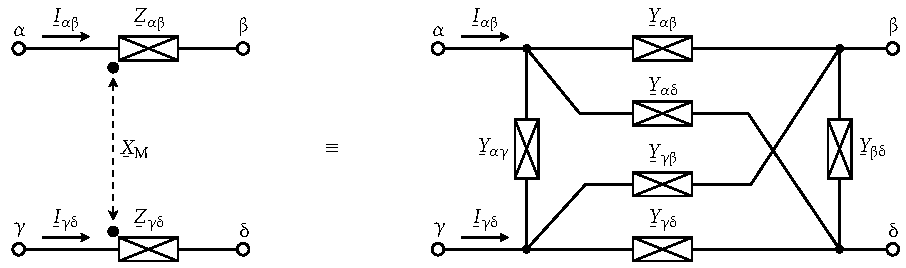
\includegraphics{Imatges/Cap-ResXarxElec-Acoblament.pdf}
   \caption{Circuit equivalent de dues branques acoblades magn\`{e}ticament} \label{pic:equiv_acobl}
\end{figure}

Els valors de les admit\`{a}ncies d'aquest circuit equivalent
s\'{o}n:\index{acoblament magn\`{e}tic!circuit equivalent}

\parbox{15cm}
{ \begin{align*}
   \cmplx{Y}_{\alphaup\betaup} &= \frac{\cmplx{Z}_{\gammaup\deltaup}}{\cmplx{Z}_{\alphaup\betaup}\, \cmplx{Z}_{\gammaup\deltaup}-\cmplx{X}\ped{M}^2} &
   \cmplx{Y}_{\alphaup\gammaup} &= \cmplx{Y}_{\betaup\deltaup} = \frac{\cmplx{X}\ped{M}}{\cmplx{Z}_{\alphaup\betaup}\, \cmplx{Z}_{\gammaup\deltaup}-\cmplx{X}\ped{M}^2} \\[1.5ex]
   \cmplx{Y}_{\gammaup\deltaup} &= \frac{\cmplx{Z}_{\alphaup\betaup}}{\cmplx{Z}_{\alphaup\betaup}\, \cmplx{Z}_{\gammaup\deltaup}-\cmplx{X}\ped{M}^2} &
   \cmplx{Y}_{\alphaup\deltaup} &= \cmplx{Y}_{\gammaup\betaup} = \frac{-\cmplx{X}\ped{M}}{\cmplx{Z}_{\alphaup\betaup}\, \cmplx{Z}_{\gammaup\deltaup}-\cmplx{X}\ped{M}^2}
\end{align*} }
\hfill
\parbox{1cm}{\begin{align}\end{align}}

Un cop hem resolt la xarxa i hem trobat els potencials dels quatre
nusos $\mcmplx{V}\ped{N}(\alphaup)$, $\mcmplx{V}\ped{N}(\betaup)$,
$\mcmplx{V}\ped{N}(\gammaup)$ i $\mcmplx{V}\ped{N}(\deltaup)$, podem
trobar els dos corrents $\cmplx{I}_{\alphaup\betaup}$ i
$\cmplx{I}_{\gammaup\deltaup}$, a partir de les expressions seg\"{u}ents:
\begin{subequations}
\begin{align}
    \cmplx{I}_{\alphaup\betaup} &=  \frac{[\mcmplx{V}\ped{N}(\alphaup) - \mcmplx{V}\ped{N}(\betaup)] \, \cmplx{Z}_{\gammaup\deltaup} - [\mcmplx{V}\ped{N}(\gammaup) - \mcmplx{V}\ped{N}(\deltaup)] \,
    \cmplx{X}\ped{M}}{\cmplx{Z}_{\alphaup\betaup}\,
    \cmplx{Z}_{\gammaup\deltaup}-\cmplx{X}\ped{M}^2} \label{eq:i_ab}
    \\[1.5ex]
    \cmplx{I}_{\gammaup\deltaup} &= \frac{[\mcmplx{V}\ped{N}(\gammaup) - \mcmplx{V}\ped{N}(\deltaup)] \, \cmplx{Z}_{\alphaup\betaup} - [\mcmplx{V}\ped{N}(\alphaup) - \mcmplx{V}\ped{N}(\betaup)] \,
    \cmplx{X}\ped{M}}{\cmplx{Z}_{\alphaup\betaup}\,
    \cmplx{Z}_{\gammaup\deltaup}-\cmplx{X}\ped{M}^2} \label{eq:i_gd}
\end{align}
\end{subequations}

El cas que hem vist fins ara, \'{e}s el m\'{e}s general de tots els
possibles, ja que suposa que els quatre nusos $\alphaup$, $\betaup$,
$\gammaup$ i $\deltaup$ s\'{o}n diferents entre si. Es pot presentar el cas,
no obstant, on dos nusos siguin en realitat el mateix, en tenir les
dues branques acoblades magn\`{e}ticament, un extrem connectat al mateix
nus; en aquest cas el circuit equivalent resultant es pot derivar
del corresponent al cas general de forma senzilla.

Si suposem, per exemple, que les dues branques de la Figura
\vref{pic:equiv_acobl} estiguessin unides pels extrems de la dreta,
\'{e}s a dir $\betaup\equiv\deltaup$, en aquest cas l'admit\`{a}ncia entre
$\alphaup$ i $\gammaup$ seria $\cmplx{Y}_{\alphaup\gammaup}$, l'admit\`{a}ncia
entre $\betaup$ i $\deltaup$ desapareixeria, l'admit\`{a}ncia entre $\alphaup$
i $\betaup$ seria $\cmplx{Y}_{\alphaup\betaup} +
\cmplx{Y}_{\alphaup\deltaup}$, i finalment, l'admit\`{a}ncia entre $\gammaup$
i $\betaup$ seria $\cmplx{Y}_{\gammaup\betaup} +
\cmplx{Y}_{\gammaup\deltaup}$. Els corrents $\cmplx{I}_{\alphaup\betaup}$ i
$\cmplx{I}_{\gammaup\deltaup}$, es calcularien tamb\'{e} amb les equacions
\eqref{eq:i_ab} i \eqref{eq:i_gd}, tenint en compte que
$\mcmplx{V}\ped{N}(\betaup)\equiv\mcmplx{V}\ped{N}(\deltaup)$.

\section{Circuits equivalents Th\'{e}venin i Norton} \index{teorema!de Th\'{e}venin} \index{teorema!de Norton} \index{metode@m\`{e}tode dels nusos!circuits equivalents Th\'{e}venin i Norton}\label{sec:xarxes_Zth}

\index{matriu!d'imped\`{a}ncies de nus $\mcmplx{Z}\ped{N}$}Per trobar el
circuit equivalent Th\'{e}venin o Norton entre dos nusos qualssevol
d'una xarxa, ens cal el vector de potencials de nus
$\mcmplx{V}\ped{N}\{n\}$, obtingut segons s'ha descrit en els
apartats anteriors, i la matriu d'imped\`{a}ncies de nus
$\mcmplx{Z}\ped{N}\{n\times n\}$; aquesta matriu est\`{a} definida per
la relaci\'{o} seg\"{u}ent:
\begin{equation}
   \mcmplx{Z}\ped{N} = \mcmplx{Y}\ped{N}^{-1}
\end{equation}

A partir del vector $\mcmplx{V}\ped{N}$ i de la matriu
$\mcmplx{Z}\ped{N}$, podem trobar la font de tensi\'{o} i la imped\`{a}ncia
Th\'{e}venin equivalents entre dos nusos qualssevol.

La tensi\'{o} Th\'{e}venin $\cmplx{E}\ped{Th}^{(\alphaup,0)}$ i la imped\`{a}ncia
Th\'{e}venin $\cmplx{Z}\ped{Th}^{(\alphaup,0)}$, entre  un nus qualsevol
$\alphaup$ i el nus de refer\`{e}ncia 0, s'obtenen amb les equacions
seg\"{u}ents:
\begin{align}
    \cmplx{E}\ped{Th}^{(\alphaup,0)} &= \mcmplx{V}\ped{N}(\alphaup) \\
    \cmplx{Z}\ped{Th}^{(\alphaup,0)} &= \mcmplx{Z}\ped{N}(\alphaup,\alphaup)
\end{align}

La tensi\'{o} Th\'{e}venin $\cmplx{E}\ped{Th}^{(\alphaup,\betaup)}$ i la
imped\`{a}ncia Th\'{e}venin $\cmplx{Z}\ped{Th}^{(\alphaup,\betaup)}$, entre dos
nusos qualssevol $\alphaup$ i $\betaup$, s'obtenen amb les equacions
seg\"{u}ents:
\begin{align}
    \cmplx{E}\ped{Th}^{(\alphaup,\betaup)} &= \mcmplx{V}\ped{N}(\alphaup) - \mcmplx{V}\ped{N}(\betaup) \\
    \cmplx{Z}\ped{Th}^{(\alphaup,\betaup)} &= \mcmplx{Z}\ped{N}(\alphaup,\alphaup) +
    \mcmplx{Z}\ped{N}(\betaup,\betaup) - \mcmplx{Z}\ped{N}(\alphaup,\betaup) -
    \mcmplx{Z}\ped{N}(\betaup,\alphaup)
\end{align}

A partir d'aquests valors podem calcular els valors del circuit Norton equivalent, utilitzant l'equaci\'{o} \eqref{eq:Thevenin-Norton} de la p\`{a}gina \pageref{eq:Thevenin-Norton}.


\begin{exemple}
Continuant amb el circuit de la Figura \vref{pic:metode_nusos}, es
tracta de trobar els circuits Th\'{e}venin i Norton equivalents de la
xarxa, entre els nusos 1 i 2.

El vector $\mcmplx{V}\ped{N}$ \'{e}s el calculat a la p\`{a}gina \pageref{eq:vn_exemp}.

Trobem a continuaci\'{o} la matriu $\mcmplx{Z}\ped{N}$, a partir de la matriu $\mcmplx{Y}\ped{N}$
calculada a la p\`{a}gina \pageref{eq:yn}:
\[
   \mcmplx{Z}\ped{N} =
   60 \cdot \begin{pmatrix}
            9 - \ju 4 & -3 + \ju 8 \\
            3 + \ju 8 & 9 - \ju 28
      \end{pmatrix} ^{-1} =
   \frac{1}{202} \cdot \begin{pmatrix}
         1445 + \ju 310 & 415 + \ju 110 \\
         415 + \ju 110 & 245 + \ju 430
   \end{pmatrix}\unit{\ohm}
\]

Els valors del circuit Th\'{e}venin equivalent que busquem s\'{o}n:
\begin{align*}
   \cmplx{E}\ped{Th}^{(1,2)} &= \frac{15430 + \ju 2295}{101} - \frac{3390 + \ju 2085}{101} =
   \frac{12040 + \ju 210}{101}\unit{V} \\[2ex]
   \cmplx{Z}\ped{Th}^{(1,2)} &= \frac{1445 + \ju 310}{202} + \frac{245 + \ju 430}{202} -
   2\cdot\frac{415 + \ju 110}{202} = \frac{430 + \ju 260}{101}\unit{\ohm}
\end{align*}

Els valors del circuit Norton equivalent que busquem s\'{o}n:
\begin{align*}
   \cmplx{J}\ped{No}^{(1,2)} &= \frac{\cmplx{E}\ped{Th}^{(1,2)}}{\cmplx{Z}\ped{Th}^{(1,2)}} =
   \frac{\frac{12040 + \ju 210}{101}\unit{V}}{\frac{430 + \ju 260}{101}\unit{\ohm}} =
   \frac{518 - \ju 301}{25}\unit{A} \\[2ex]
   \cmplx{Y}\ped{No}^{(1,2)} &= \frac{1}{\cmplx{Z}\ped{Th}^{(1,2)}} =
   \frac{1}{\frac{430 + \ju 260}{101}\unit{\ohm}} = \frac{43 - \ju 26}{250}\unit{S}
\end{align*}

\end{exemple}
